% === II. Latar Belakang Ide Perangkat Lunak ===
\secbox{II.}{Latar Belakang Ide Perangkat Lunak}

Krisis kesehatan mental telah menjadi isu kesehatan publik global, dengan hampir 1,1 miliar jiwa (1 dari 7 orang) hidup dengan gangguan psikologis, termasuk gangguan kecemasan dan depresi (Dhia Tawakalna \& Junta Zeniarja, 2026; Gong et al., 2026). Seperti yang terlihat pada Gambar 1, sekitar 9,8\% penduduk di Indonesia mengalami gangguan psikologis, namun hanya 2,5\% yang memperoleh layanan konseling profesional akibat rendahnya literasi kesehatan mental (Dhia Tawakalna \& Junta Zeniarja, 2026). Kondisi ini secara signifikan memengaruhi Generasi Z (10--24 tahun), yang merupakan periode munculnya sekitar 75\% gangguan mental pertama kali (Casey Annie E., 2024). Berbagai studi juga menunjukkan bahwa 84\% Generasi Z menganggap kesehatan mental sebagai krisis nasional, 91\% pernah mengalami stres, sementara 60\% merasa kewalahan menghadapi berbagai tekanan global, tetapi hanya separuh yang mengetahui tempat memperoleh bantuan psikologis (Arrahmi Thahir et al., 2023; Casey Annie E., 2024, 2025; UNICEF, 2025).

\begin{figure}[H]
    \centering
    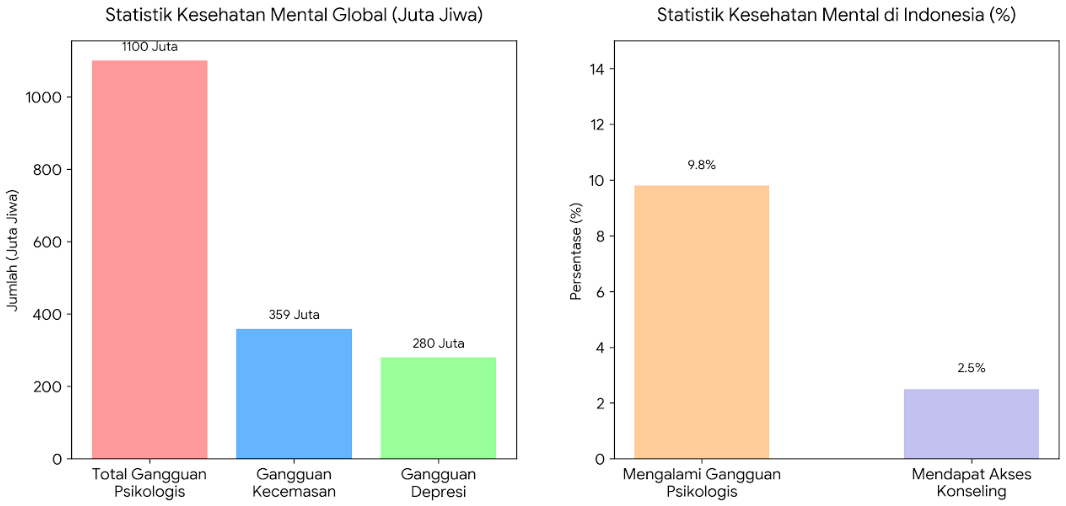
\includegraphics[width=0.85\textwidth]{images/bab2/fig1_statistik.png}
    \caption{Statistik Kesehatan Mental}
\end{figure}

Kerentanan tersebut dipengaruhi oleh penggunaan internet dan media sosial secara intensif yang memicu isolasi sosial, kesepian, gangguan tidur, perundungan siber, serta fenomena \textit{Fear of Missing Out} (FOMO), dan diperparah oleh tekanan ekonomi, akademik, kecemasan iklim, hingga kekhawatiran terhadap otomatisasi pekerjaan oleh kecerdasan buatan (Arrahmi Thahir et al., 2023; Fadli, 2024). Tanpa intervensi dini, kondisi ini berdampak pada penurunan konsentrasi belajar, penarikan diri dari lingkungan sosial, serta peningkatan risiko bunuh diri yang menjadi salah satu penyebab utama kematian pada kelompok usia 15--29 tahun (Arrahmi Thahir et al., 2023; Casey Annie E., 2025; Fadli, 2024).

Meskipun kebutuhan akan pendampingan psikologis semakin mendesak, akses terhadap layanan profesional masih terhambat oleh keterbatasan jumlah psikolog, tingginya biaya terapi, serta stigma sosial terhadap pencari bantuan (Arrahmi Thahir et al., 2023; Dhia Tawakalna \& Junta Zeniarja, 2026). Di sisi lain, aplikasi kesehatan mental berbasis aturan (\textit{rule-based}) belum mampu memahami percakapan secara empatik (Dhia Tawakalna \& Junta Zeniarja, 2026). Sementara itu, pemanfaatan Large Language Model (LLM) generatif tunggal berisiko memicu halusinasi medis (Fransson, 2026), tidak memiliki memori percakapan jangka panjang antar-sesi (Packer et al., 2024), serta membebankan pencatatan diari secara manual yang sering diabaikan pengguna. Tinjauan literatur juga menunjukkan adanya kesenjangan keselamatan (\textit{safety gap}), di mana 48,28\% chatbot kesehatan mental komersial gagal memberikan respons yang memadai terhadap situasi krisis bunuh diri (Elbarbary et al., 2026).

Guna memastikan keabsahan ilmiah dan efektivitas dalam mengukur kondisi emosional pengguna, tim pengembang telah melakukan studi pendahuluan dan wawancara klinis bersama \textbf{Qori Fanani, M.Psi., Psikolog} (Petugas Poliklinik Politeknik Negeri Malang dan Dosen Psikologi Universitas Kepanjen). Berdasarkan hasil konsultasi tersebut, instrumen \textbf{DASS-21 (\textit{Depression Anxiety Stress Scale 21})} direkomendasikan dan divalidasi sebagai kerangka kerja psikometris utama dalam LUNA. Kerangka DASS-21 memungkinkan sistem mengukur tiga indikator psikologis utama—yaitu tingkat depresi, kecemasan (\textit{anxiety}), dan stres—secara terpisah melalui perhitungan skor yang terukur, sehingga LUNA mampu membedakan tingkat distres emosional non-klinis secara akurat (Dokumentasi wawancara disajikan pada Lampiran 6).

Berdasarkan permasalahan tersebut, penulis mengusulkan LUNA (Listening, Understanding, Nurturing Assistant) sebagai platform pendamping kesehatan mental berbasis Multi-Agent AI bagi Generasi Z yang mengintegrasikan enam fitur utama, yaitu \textit{Personalized Mental Health Support}, \textit{Automatic Diary Generation}, \textit{Long-term Conversation Memory}, \textit{Emotion \& Mental Risk Analysis}, \textit{Early Mental Crisis Detection}, dan \textit{Voice Conversation}. Kebaruan LUNA terletak pada arsitektur Multi-Agent AI yang mengorkestrasi agen terapis, pembuat diari, penilai risiko krisis, dan pengelola memori berbasis RAG, sehingga mampu memberikan pendampingan yang lebih personal, berkelanjutan, dan aman dibandingkan chatbot berbasis LLM tunggal. LUNA selaras dengan subtema AI in Health and Well-being AI untuk meningkatkan akses pendampingan psikologis awal dan deteksi dini krisis emosional.
